\structure{ХОД РАБОТЫ}

В проекте был написан класс для решения игр с моделью информационного противоборства в социальных сетях.

Пример запуска программы:

\begin{codelisting}[language=Bash]
    go run cmd/rk3/main.go
\end{codelisting}

Сгенерируем стохастическую матрицу доверия для 10 агентов
случайным образом при помощи написанной программы. Вывод программы представлен на рисунке~\ref{fig:fig01}

\begin{figure}
  \centering
  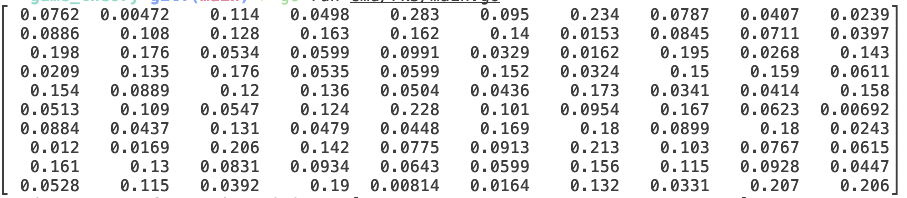
\includegraphics[scale=0.5]{../../artifacts/rk3/1.png}
  \caption{Случайная матрица доверя 10x10}
  \label{fig:fig01}
\end{figure}

Сгенерированный вектор изначальных мнений агентов представлен на рисунке~\ref{fig:fig02}.

\begin{figure}
  \centering
  
\includegraphics[scale=0.6]{../../artifacts/rk3/2.png}
  \caption{Вектор изначальных мнений агентов}
  \label{fig:fig02}
\end{figure}

\section{Нахождение итогового мнения агентов без влияния}

Применим алогоритм согласно формуле (1) с точностью $\mathcal E = 10^{-6}$.

\begin{equation}
\mathbf{x}(t) = A \mathbf{x}(t - 1).
\end{equation}
где $A$ -- случайная матрица доверия, а $x(0)$ -- вектор изначальных мнений агентов.

Спустя 11 итераций алгоритм остановится, так как разница между двумя последними векторами в каждой
координате оказались меньше $10^{-6}$. Вывод итераций представлен на рисунке~\ref{fig:fig03}.

\begin{figure}
  \centering
  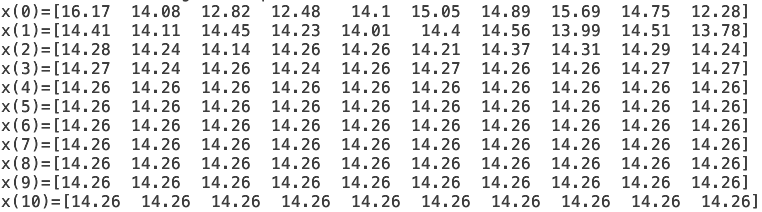
\includegraphics[scale=0.6]{../../artifacts/rk3/3.png}
  \caption{Итерации примененного алоритма}
  \label{fig:fig03}
\end{figure}

После взаимодействия агентов, вектор мнений сходится к значению $14.26$.

Результирующая матрица доверия представлена на рисунке~\ref{fig:fig04}.

\begin{figure}
  \centering
  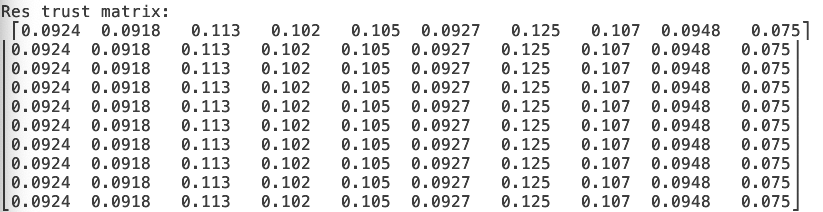
\includegraphics[scale=0.6]{../../artifacts/rk3/4.png}
  \caption{Результирующая матрица доверия}
  \label{fig:fig04}
\end{figure}

\section{Решение игры с информационным влиянием}

Индексы агентов влияния для 2-х игроков представлены на рисунке~\ref{fig:fig05}.

\begin{figure}
  \centering
  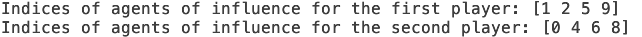
\includegraphics[scale=0.6]{../../artifacts/rk3/5.png}
  \caption{Индексы агентов влияния для 2-х игроков}
  \label{fig:fig05}
\end{figure}

Случайные изначальные мнения для двух игроков представлены на рисунке~\ref{fig:fig06}.

\begin{figure}
  \centering
  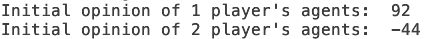
\includegraphics[scale=0.6]{../../artifacts/rk3/6.png}
  \caption{Случайные изначальные мнения для 2-х игроков}
  \label{fig:fig06}
\end{figure}

Аналогично первому пункту, применим алгоритм согласно формуле (1) и остановимся, когда точность не будет
превышать $10^{-6}$. Итерации алгоритма представлены на рисунке~\ref{fig:fig07}.

\begin{figure}
  \centering
  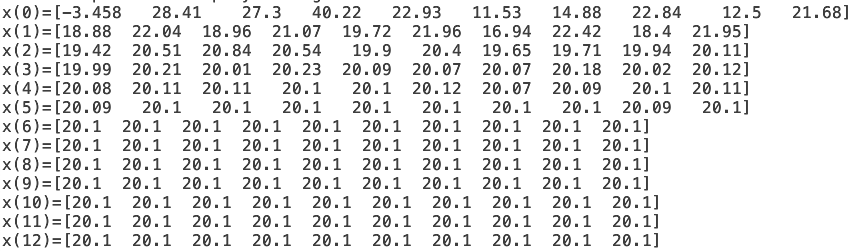
\includegraphics[scale=0.6]{../../artifacts/rk3/7.png}
  \caption{Итерации алгоритма}
  \label{fig:fig07}
\end{figure}

После взаимодействия агентов, вектор мнений сходится к значения, показанный на рисунке~\ref{fig:fig08}

\begin{figure}
  \centering
  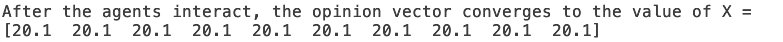
\includegraphics[scale=0.6]{../../artifacts/rk3/8.png}
  \caption{Вектор мнений}
  \label{fig:fig08}
\end{figure}

Результирующая матрица доверия представлена на рисунке~\ref{fig:fig09}.

\begin{figure}
  \centering
  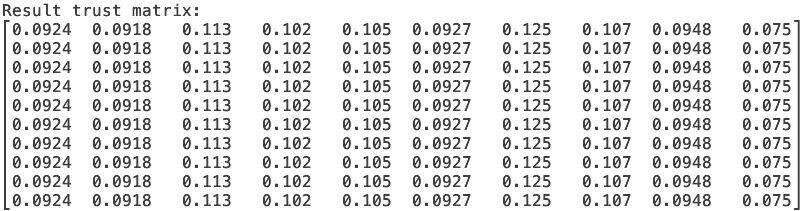
\includegraphics[scale=0.6]{../../artifacts/rk3/9.png}
  \caption{Результирующая матрица доверия}
  \label{fig:fig09}
\end{figure}

Получим $r_f$, $r_s$ (см. рисунок~\ref{fig:fig10}).

\begin{figure}
  \centering
  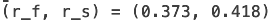
\includegraphics[scale=0.6]{../../artifacts/rk3/10.png}
  \caption{Полученные значения $r_f$, $r_s$}
  \label{fig:fig10}
\end{figure}

Для целевых функций игроков:

\[
\Phi_f(u,v) = a(r_fu + r_sv) - b(r_fu + r_sv)^2 - g_f \frac{u^2}{2}
\]

\[
\frac{\partial \Phi_f(u,v)}{\partial u} = a r_f - 2b(r_fu + r_sv)r_f - g_f u
\]

\[
\Phi_s(u,v) = c(r_fu + r_sv) - d(r_fu + r_sv)^2 - g_s \frac{v^2}{2}
\]

\[
\frac{\partial \Phi_s(u,v)}{\partial v} = c r_s - 2d(r_fu + r_sv)r_s - g_s v
\]

Решаем систему:
\[
\begin{cases}
a r_f - 2b(r_fu + r_sv)r_f - g_f u = 0 \\
c r_s - 2d(r_fu + r_sv)r_s - g_s v = 0
\end{cases}
\]

Из первого уравнения:
\begin{equation}
v = \frac{u(-2b r_f^2 - g_f) + a r_f}{2b r_f r_s}
\end{equation}

Из второго уравнения:
\begin{equation}
u = \frac{2 a d r_f r_s^2 + a r_f g_s - 2 b c r_f r_c^2}{g_f g_s + 2 b r_f^2 g_s + 2 d r_s^2 g_f}
\end{equation}

Подставим числа из варианта и получим уравнения, представленные на рисунке~\ref{fig:fig11}.

\begin{figure}
  \centering
  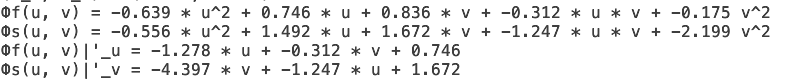
\includegraphics[scale=0.6]{../../artifacts/rk3/11.png}
  \caption{Полученные уравнения}
  \label{fig:fig11}
\end{figure}

Согласно (2) и (3) получим ответы.

\[
  \begin{cases}
  u = 0.527 \\
  v = 0.231
  \end{cases}
\]

Точка утопии:

\[
  X_{max} = 0.48
\]

Оптимальные мнения:

\begin{align*}
  X_{max f} = 1 \\
  X_{max s} = 0.5
\end{align*}

Найдем расстояния:

\begin{align*}
  \Delta_{x_f} &= 0.52 \\
  \Delta_{x_s} &= 0.02
\end{align*}

Как мы видим, $\Delta_{x_f} > \Delta{x_s}$, поэтому выиграл второй игрок.
